\chapter{MiCS Implementation}
	In this chapter, the implementation of MiCS will be described. It will start out by discussing the different types that can be used in MiCS and then describe each of the five stages when generating JavaScript from C\# as explained in section \ref{sec:workflow_overview}. For clarity purposes, the third stage (Building + Mapping to Script\# AST) is divided into two different sections.


\section{Initializing MiCS} % (fold)
\label{sec:initializing_mics}

Før MiCS kan begynde at konvertere C# til JavaScript, skal de nødvendige ressourcer konstrueres. 
Det er det første der gøres, inden validering, konvertering og injektion finder sted.
De ressourcer som skal initialiserers, er TypeManager'ne.
	Indeholder CompilationUnit, Semantiske Modeller, Core Mappings, MixedSide members (Alt med MixedSide) og ClientSide members (Alt med ClientSide / DOM Types) 


* How does the MiCS project know what code to generate JavaScript from? // Forklares i afsnit om Roslyn
* Gathering server side source code (currently from filepaths). // Forklares i WorkFlow afsnit?
* Adding ScriptSharp DOM classes to semantic model.
* Adding C# msCoreLib (System) and System.Text.RegularExpressions namespace to C# semantic model.



% section initializing_mics (end)

\section{Validating Mixed and Client Side Code} % (fold)
\label{sec:syntax_tree_validation}
	% As we only support a fairly limited set of C\#’s built-in constructs and types, it is important to make sure that users only make use of those that we are able to map to Script\#. Should users utilise one of the constructs or types that we are not able to map, this should be pointed out with an understandable error message. It should not be left to the users to debug or understand a Roslyn or Script\# exception. Furthermore, it is important to make sure that users use their own code correctly. The remainder of this section will describe how a Validator class is used to achieve this.

	Before the Roslyn AST is mapped to Script\# it is necessary to verify that types and their members are used correcly. This is handled by the \texttt{Validator} class. If the developer only uses .NET types that we can map to Script\# and adhere to the Mixed Side Principle, the validation passes. The remainder of this section focus on how this validation is done.
	%Understanding “correct usage of .NET built-in types and members” is straightforward; it means that users are only allowed to use the types and members that can be mapped correctly to Script\#. How this is achieved is described later in this section. However, “correct usage of the types defined by the users themselves” requires some explanation. For this, the MixedSide Principle is introduced.

%To explain correct usage of types and their members, it is beneficial to divide them into two categories; types that are built into the .NET platform and types developers define themselves.



There are essentially three situations in which it is necessary to verify correct usage of types and members.

\begin{itemize}
	\item Object creation; when an instance of a type is created, it is necessary to check the type in question can be mapped.
	\item When members on type instances are accessed; it is then necessary to check first if the type can be mapped, then if the type has a member corresponding to the one being accessed.
	\item Invocation of methods on .NET core types; it is then necessary to check whether the invocation is done correctly, using the correct arguments and return type. Normally, the C\# compiler complains if an invocation is done using an incorrect signature, but as the interface between .NET core types and Script\# core types does not always match, it is important to make sure that the Script\# core type has a member with the corresponding arguments and return type. An invocation that is perfectly legal on .NET core types might be illegal on Script\# core types.
\end{itemize}

The \texttt{Validator} class extends Roslyn's \texttt{SyntaxWalker} class and it is thus able to traverse syntax nodes. The \texttt{Validator} takes a syntax tree that holds the source code to be validated, a string containing an attribute name (''MixedSide'' or ''ClientSide'') that decides what methods to validate, and a structure of types and members that can legally be used without violating the Mixed Side Principle. The \texttt{Validator} works by looking for classes in the syntax tree that contains methods annotated with the given attribute name and validates the body of these methods against the provided structure of allowed members.

The nature of the \texttt{Validator} requires the syntax tree to be validated twice. This is done by creating two instances of the Validator class, a \emph{MixedSide Validator} and a \emph{ClientSide Validator}, and validating them both. 
The MixedSide validator will do \emph{MixedSide validation} and the ClientSide validator will do \emph{ClientSide validation}:

\begin{itemize}
	\item \emph{MixedSide validation} requires validating all the \texttt{MixedSide} methods against a structure containing all \texttt{MixedSide} types and their members
	\item \emph{ClientSide validation} requires validating all the \texttt{ClientSide} methods against a structure containing all \texttt{ClientSide} types and members, \texttt{MixedSide} types and members and Script\# DOM types and members.
\end{itemize}


The Validation process is best explained by looking at an example. Consider a syntax tree holding the simple piece of code shown in figure \ref{fig:mixedSideValidationExample}. The methods of \texttt{ExampleClass} are subjects for MixedSide validation.

\begin{figure}[H]
	\begin{lstlisting}[language=CSharp,classoffset=1,morekeywords={ExampleClass,AnotherExampleClass,MixedSide}]
namespace ExampleNamespace
{
  public class ExampleClass
  {
  	[MixedSide]
  	public void ExampleMethod()
  	{
  		var a = new AnotherExampleClass();
  	}
  }
  
  public class AnotherExampleClass
  {
  	[MixedSide]
  	public void AnotherExampleMethod() { }
  }
}
	\end{lstlisting}
	\caption{Code subject to MixedSide validation}
	\label{fig:mixedSideValidationExample}
\end{figure}		

The MixedSide Validator traverses the syntax tree and discovers the \texttt{ExampleClass} class. It then finds all of the class' methods and checks if they have the \texttt{MixedSide} attribute. When a method annotated with the MixedSide attribute is found, the MixedSide Validator visits it straight away, as shown in Figure \ref{fig:ValidatorVisitClassDeclaration}. 

\begin{figure}[H]
	\begin{lstlisting}[language=CSharp,classoffset=1,morekeywords={ClassDeclarationSyntax,SyntaxKind,MethodDeclarationSyntax,List}]
/// <summary>
/// Visits the ClassDeclaration and determines wether its members should be validated
/// </summary>
public override void VisitClassDeclaration(ClassDeclarationSyntax @class)
{
  List<MethodDeclarationSyntax> methods = @class.DescendantNodes().Where(a => a.Kind == SyntaxKind.MethodDeclaration);
  bool visit = false;

  foreach (var method in methods)
  {
    visit = ((MethodDeclarationSyntax)method).HasAttribute(attributeName);

    if (visit)
      VisitMethodDeclaration((MethodDeclarationSyntax)method);
  }
}
	\end{lstlisting}
	\caption{Visiting a \texttt{ClassDeclarationSyntax} and deciding whether or not its methods should be validated}
	\label{fig:ValidatorVisitClassDeclaration}
\end{figure}


The first method visited is the \texttt{ExampleMethod()} method. The first statement of the method contains an object creation expression and the MixedSide Validator now needs to check if the object creation is legal. It is legal either if the created object is a supported core type, or if the created object is MixedSide type defined by the developer.



As the type exists in the allowed members structure (shown in figure \ref{fig:mixedSideValidationExample}) the object creation is legal and the traversal continues. If it had not existed in the allowed member structure (this could happen if it had been ClientSide), and had not been a supported core type, the MixedSide Principle would have been violated, and an exception of type \texttt{MixedSidePrincipleViolatedException} had been thrown.

The validation of a member access is done in a very similar way, only checking if the member exists in the allowed-members structure or in the core mapping as well.

As mentioned earlier, it is important to validate invocation on core types. This is done using the \texttt{VerifyCorrectUseOfSupportedCoreType} method on the \texttt{TypeManager}. This method first checks if the given invocation is done on a core type, and subsequently uses the Core Mapping Specification (as discussed in section \ref{sub:type_mapping}) to verify that we are able to map the invocation to ScriptSharp.
		



		% When an invocation is visited, the \texttt{TypeManager} is asked to 
		% TODO: Write about how invociations are validated: Only core types need to be validated (with arguments and return types), as user types will automatically be validated by the compiler.


% \begin{lstlisting}[language=CSharp,classoffset=1,morekeywords={TextBox,Panel,CheckBox, Button}]
% TextBox NameBox = new TextBox() { ID = "name", Text = "Name" };
% Panel CheckBoxGroup = new Panel();
% CheckBox SnailMailCheck = new CheckBox() { ID = "dmSnailmail", Text = "Snail Mail" };
% CheckBox EmailCheck = new CheckBox() { ID = "dmEmail", Text = "E-Mail" };
% TextBox AddressBox = new TextBox() { ID = "address", Text = "Address" };
% TextBox ZipcodeBox = new TextBox() { ID = "zipcode", Text = "Zip Code" };
% TextBox EmailBox = new TextBox() { ID = "email", Text = "E-mail" };
% TextBox PhoneBox = new TextBox() { ID = "phone", Text = "Phone" };
% Button SubmitButton = new Button() { Text = "Register" };
% \end{lstlisting}






	
	% subsection validating (end)
% section syntax_tree_validation (end)

\section{Mapping to Script\# AST} % (fold)
\label{sec:mapping_to_scriptsharp_ast}
	When converting the validated Roslyn AST to its corresponding Script\# AST, a logical division of the process has been made. 

	\begin{itemize}
		\item Mapping a Roslyn AST node to its equivalent Script\# AST node
		\item Building a Script\# AST from all the mapped nodes
	\end{itemize}

	It is important to realize that the mapping is a sub process of the building process. The mapping is discussed in this section. 

	\subsection{Expressions, Statements and Symbols} % (fold)
	\label{sub:subsection_mapping_to_scriptsharp_expressions_statements_and_symbols}
		The mapping of Expressions, Statements and Symbols is implemented in three classes (ExpressionMapper.cs, StatementMapper.cs and SymbolMapper.cs). The three classes are logically divided (and named) after the kind of Script\# AST node they map to. 

		\begin{figure}[H]
			\begin{center}
				\centerline{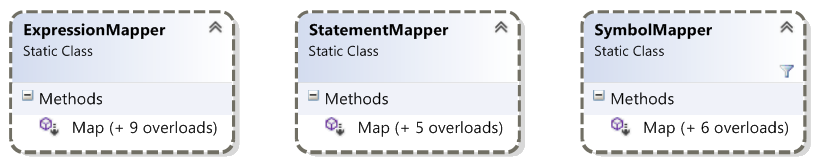
\includegraphics[width=14cm]{resources/images/MapperClasses.png}}
			\end{center}
			\caption{Classes that define extension methods for mapping Roslyn AST nodes to Script\# AST nodes.}
			\label{mapperClasses}
		\end{figure}

		Mapping of AST nodes is somewhat straightforward as most Roslyn AST nodes have an equivalent Script\# AST node. E.g. a Roslyn return statement node maps to a Script\# return statement etc. The three mapper classes define \texttt{Map(...)} extension methods to the Roslyn node objects they map from (see example figures \ref{returnStatementMap} and \ref{conditionaleExpressionMap}).

		\begin{figure}[H]
			\begin{center}
				\centerline{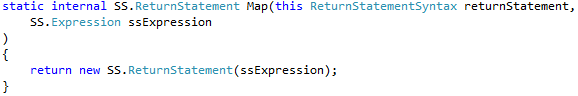
\includegraphics[width=14cm]{resources/images/ReturnStatementMap.png}}
			\end{center}
			\caption{Extension method that maps Roslyn return statement to Script\# return statement.}
			\label{returnStatementMap}
		\end{figure}

		\begin{figure}[H]
			\begin{center}
				\centerline{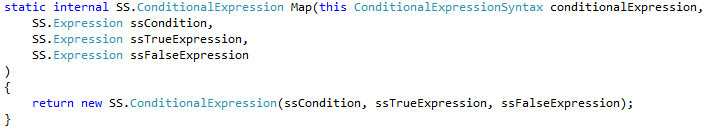
\includegraphics[width=14cm]{resources/images/ConditionalExpressionMap.png}}
			\end{center}
			\caption{Extension method that maps Roslyn conditional expression to Script\# conditional expression.}
			\label{conditionaleExpressionMap}
		\end{figure}
	% subsection subsection_mapping_to_scriptsharp_expressions_statements_and_symbols (end)

	\subsection{Type Mapping} % (fold)
	\label{sub:type_mapping}
		Roslyn type symbols are mapped to Script\# type symbols using the \texttt{SymbolMapper}’s \texttt{Map(...)} extension method created for the Roslyn \texttt{TypeSymbol}. The mapping of type symbols from Roslyn to Script\# can be somewhat confusing since there are the different kinds of types (illustrated in figure \ref{typesOverview}) and there are some special cases (such as \texttt{null} which is mapped to the type \texttt{Object} in JavaScript). To illustrate the functionality of the \texttt{TypeSymbol} \texttt{Map(...)} method we have created the flowchart in figure \ref{typeMappingFlowchart}.

			\begin{figure}
			\begin{center}
					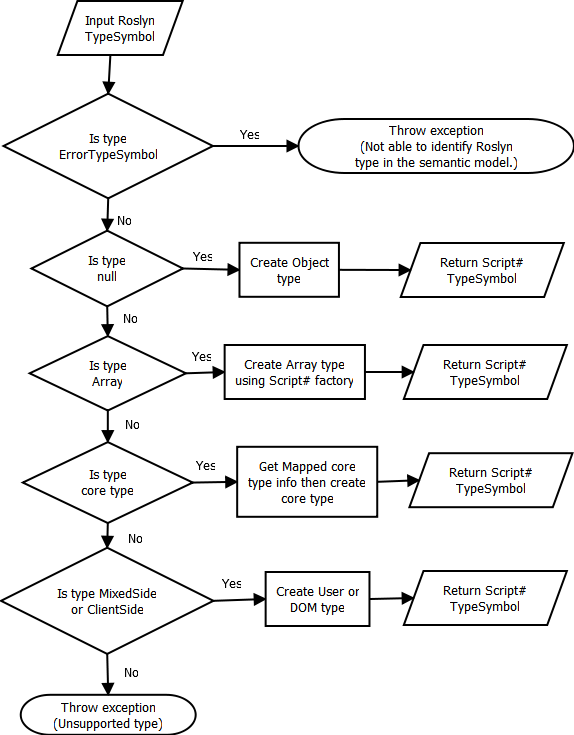
\includegraphics[width=14cm]{resources/images/TypeMappingFlowchart.png}
					\end{center}
				\caption{The type mapping process performed in \texttt{SymbolMapper.Map(this TypeSymbol typeSymbol)} extension method.}
				\label{typeMappingFlowchart}
			\end{figure}


		\subsubsection{Core Type Mapping} % (fold)
		\label{subsub:core:type_mapping}
			In contrast to using Script\# in the original manner (where the Script\# core types are used when writing code instead of the .NET core types) our project only uses the Script\# core types when mapping to the Script\# JavaScript AST. For this reason the Script\# core types are handled by its own type manager class (\texttt{ScriptSharpTypeManager.cs}). From the \texttt{ScriptSharpTypeManager} the Roslyn type symbols are retrieved before they are mapped to Script\# type symbols needed when building the Script\# AST.

			Since the .NET core types are used when writing code with MiCS and since these are mapped to the Script\# core types a mapping specification is needed. To facilitate this mapping we have created some simple classes to hold the specification (\texttt{MiCSCoreMapping.cs}, \texttt{MiCSCoreTypeMapping.cs} and \texttt{MiCSCoreMemberMapping.cs}) which can be queried using LINQ. This mapping specification contains information on the core types that we currently support. If a core type is not described in the specification then it is not supported. If the core type is found in the specification then the same pattern applies for its members. If a type member is not found then it is not supported. The mapping specification also holds information on a member’s return type, number of arguments and the arguments’ types.

			\begin{figure}[H]
					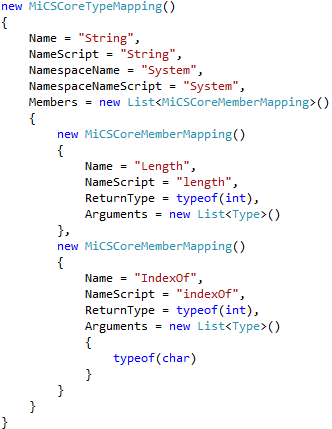
\includegraphics[width=8cm]{resources/images/InitiationOfTypeMapping.png}
				\caption{Instantiation example of a single core type (System.String) mapping specification.}
				\label{coreTypeMapping}
			\end{figure}

			An example of a core type mapping is the C\# System.String (see figure \ref{coreTypeMapping}) type which is mapped to the Script\# defined \texttt{System.String}. We are only mapping two of the String type’s members. The field \texttt{Length} which is mapped to the Script\# \texttt{String} type’s \texttt{Length} field (which is the equivalent of the JavaScript \texttt{String} object's property \texttt{length}). The second member we map is the \texttt{IndexOf(Char char)} method that returns an int. There are other \texttt{IndexOf} methods that take multiple arguments or a single argument of a different type (than \texttt{Char}) but these are not mapped in our mapping specification.

			Apart from the regular core types (i.e. the core types defined in the .NET \texttt{mscorlib.dll}) Script\# defines additional types in its \texttt{mscorlib.dll} file. One example is the regular expression class \texttt{Regex} which is of special interest as it is used in our case study. Usually the \texttt{Regex} class is placed in the \texttt{System.Text.RegularExpressions} namespace. In the Script\# \texttt{mscorlib.dll} however \texttt{Regex} is placed in the \texttt{System} namespace. The core type mapping should also express such differences in namespaces.
		% subsection subsection_name (end)
	% subsection type_mapping (end)
% section mapping_to_scriptsharp_ast (end)

\section{Building the Script\# AST} % (fold)
\label{sec:building_the_scriptsharp_ast}
	Building the Script\# AST consists of taking the mapped AST nodes and putting them together to form the Script\# AST. The builder classes uses the Roslyn infrastructure by extending the \texttt{SyntaxWalker} class which makes them capable of traversing the Roslyn AST.
	\begin{figure}[H]
		\begin{center}
			\centerline{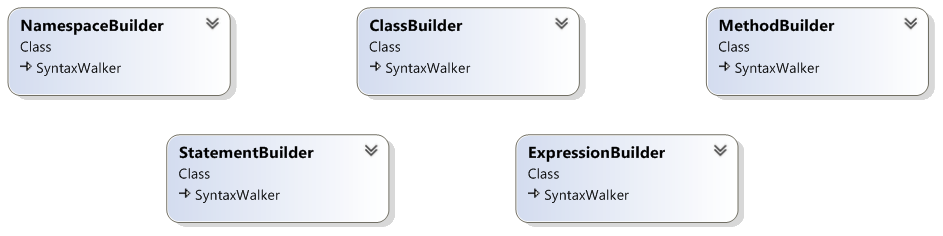
\includegraphics[width=16cm]{resources/images/BuilderClasses.png}}
		\end{center}
		\caption{Classes that build the Script\# AST by traversing the Roslyn AST and using the \texttt{Map(...)} extension methods.}
		\label{builderClasses}
	\end{figure}

	The \texttt{NamespaceBuilder} class is responsible for building all of the types contained in a namespace. This is done by instantiating a \texttt{ClassBuilder} which in turn is responsible for building all of the member methods in a class (which is done using a \texttt{MethodBuilder}). This implies that the building of the Script\# AST is done in a depth first manner (the same way the Roslyn AST is traversed).  

	\begin{figure}[H]
		\begin{center}
			\centerline{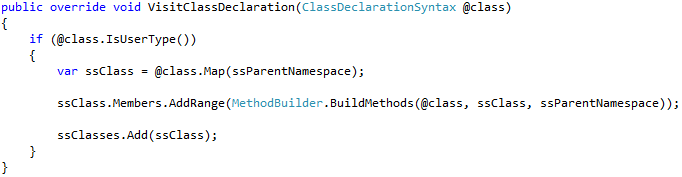
\includegraphics[width=16cm]{resources/images/VisitClassDeclaration.png}}
		\end{center}
		\caption{Empty Script\# class is created and then built by using a \texttt{MethodBuilder} to retrieve all its member methods. The \texttt{ssClasses} property on the class builder holds all the classes that will be returned to the \texttt{NamespaceBuilder} who created it.}
		\label{visitClassDeclaration}
	\end{figure}

	The \texttt{NamespaceBuilder} and \texttt{ClassBuilder} classes are somewhat trivial. The \texttt{ClassBuilder} however ensures that DOM or core types are not be mapped to Script\#. The DOM and core types doesn't need to be generated as JavaScript types because they are built in types that already exists in JavaScript.

	The \texttt{MethodBuilder} class is a little more complex. It needs to build only the methods that are mixed side or client side methods. Furthermore it needs to handle a method’s return type, arguments and body statements. 

	Likewise the \texttt{StatementBuilder} and \texttt{ExpressionBuilder} are somewhat complex as building compound statements and expressions also bares some complexity. Before a compound statement or expression can be built all its child nodes and their associated types (if any) needs to be mapped. Figure \ref{visitIfStatement} shows an if-statement AST node is built.

	\begin{figure}[H]
		\begin{center}
			\centerline{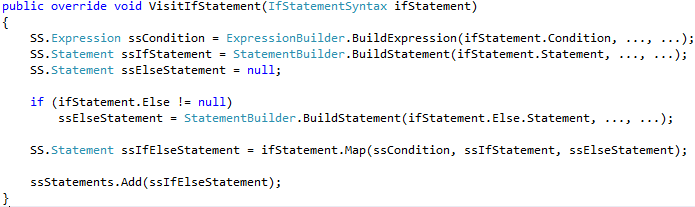
\includegraphics[width=16cm]{resources/images/VisitIfStatement.png}}
		\end{center}
		\caption{To build an if-statement node its child nodes; condition, if-block and else-block (if any) has to be built first.}
		\label{visitIfStatement}
	\end{figure}

	When a builder class is done building the node(s) are returned to the parent builder class. Once all the namespaces has been built these constitute the Script\# AST which is then passed on in the overall workflow (to script generation).
% section building_the_scriptsharp_ast (end)

\section{Script Generation} % (fold)
\label{sec:script_generation}
	Script generation is done using the Script\# infrastructure only. Specifically the \texttt{TypeGenerator} class located in the \texttt{ScriptSharp.Generator} namespace is used for this. The \texttt{MiCSManager} is responsible for instantiating the \texttt{TypeGenerator} and providing it with types from the Script\# AST. This happens in the \texttt{MiCSManager.GenerateScriptText} method.
% section script_generation (end)

\section{Integration with Web Forms} % (fold)
\label{sec:integration_with_web_forms}
	Because of the time constraint on this project integration with Web Forms has only received a minimum amount of our time. We have ensured that we could implement our case study however there should be made improvements to the Web Forms integration code which we will discuss in section \ref{ssub:integration_with_web_forms}.

	However integration with Web Forms is currently done using the \texttt{MiCSPage} class. The \texttt{MiCSPage} class inherits from the \texttt{System.Web.UI.Page} class so that it’s possible to inherit from the \texttt{MiCSPage} class in one's Code Behind file.  The \texttt{MiCSPage} class searches the specific project's file structure for C\# files, reads their content and passes this content to the \texttt{MiCSManager} who then starts the entire MiCS workflow so that the client side script will be generated. The generated script is then registered with a \texttt{ScriptManager} which is how scripts are embedded into a page from Code Behind.

	Another important aspect of integration with Web Forms is how the generated client side scripts are initially called. Client side scripts are usually initiated through DOM events such as \texttt{onload} and \texttt{onclick} which are triggered when a web page is loaded and when a button is clicked respectively. MiCS currently only supports registering a client side method on a buttons click event using our extension method \texttt{OnClientClick(…)}.

% section integration_with_web_forms (end)
